\documentclass[aspectratio=169,12pt]{beamer}
\usepackage[utf8]{inputenc}
\usepackage{graphicx}
\usepackage{tikz}
\usepackage{listings}
\usepackage{hyperref}
\usepackage{booktabs}
\usepackage{multicol}
\usepackage{xcolor}

\usetheme{Madrid}
\usecolortheme{whale}
\setbeamertemplate{navigation symbols}{}

\definecolor{codegreen}{rgb}{0,0.6,0}
\definecolor{codegray}{rgb}{0.5,0.5,0.5}
\definecolor{codepurple}{rgb}{0.58,0,0.82}
\definecolor{backcolour}{rgb}{0.95,0.95,0.92}

\lstdefinestyle{mystyle}{
    backgroundcolor=\color{backcolour},   
    commentstyle=\color{codegreen},
    keywordstyle=\color{magenta},
    numberstyle=\tiny\color{codegray},
    stringstyle=\color{codepurple},
    basicstyle=\ttfamily\footnotesize,
    breakatwhitespace=false,         
    breaklines=true,                 
    captionpos=b,                    
    keepspaces=true,                 
    numbers=left,                    
    numbersep=5pt,                  
    showspaces=false,                
    showstringspaces=false,
    showtabs=false,                  
    tabsize=2
}
\lstset{style=mystyle}

\title{Understanding Web Application Security and Attack Mitigation}
\subtitle{4-Day Comprehensive Training Program}
\author{Security Training Team}
\institute{Web Application Security Department}
\date{\today}

\begin{document}

\begin{frame}
\titlepage
\end{frame}

\begin{frame}{Training Overview}
\begin{columns}
\column{0.5\textwidth}
\textbf{Duration:} 4 Days (8 hours/day)\\
\textbf{Format:} Interactive Training\\
\textbf{Prerequisites:} Basic Web Development Knowledge
\column{0.5\textwidth}
\textbf{Learning Objectives:}
\begin{itemize}
\item Identify web application threats
\item Implement security measures
\item Understand attack methodologies
\item Apply mitigation strategies
\end{itemize}
\end{columns}
\end{frame}

\begin{frame}{Training Schedule}
\begin{table}
\centering
\begin{tabular}{ll}
\toprule
\textbf{Day} & \textbf{Topics} \\
\midrule
Day 1 & Web Application Architecture and Fundamentals \\
Day 2 & Web Application Threats and OWASP Top 10 \\
Day 3 & Web Application Hacking Methodology and Tools \\
Day 4 & Security Testing, Mitigation, and Best Practices \\
\bottomrule
\end{tabular}
\end{table}
\end{frame}

\section{Day 1: Web Application Architecture and Fundamentals}

\begin{frame}{Day 1: Agenda}
\begin{enumerate}
\item \textbf{Morning Session (4 hours)}
\begin{itemize}
\item Web Application Architecture Overview
\item Client-Side Components
\item Server-Side Components
\item Database Layer
\end{itemize}
\item \textbf{Afternoon Session (4 hours)}
\begin{itemize}
\item Component Interactions
\item Common Web Technologies
\item Security Architecture Principles
\item Hands-on Lab: Architecture Analysis
\end{itemize}
\end{enumerate}
\end{frame}

\begin{frame}{Web Application Architecture Overview}
\begin{columns}
\column{0.6\textwidth}
\textbf{Key Components:}
\begin{itemize}
\item Client-Side (Frontend)
\item Server-Side (Backend)
\item Database Layer
\item Network Infrastructure
\end{itemize}
\textbf{Architecture Patterns:}
\begin{itemize}
\item Monolithic
\item Microservices
\item Serverless
\item Progressive Web Apps
\end{itemize}
\column{0.4\textwidth}
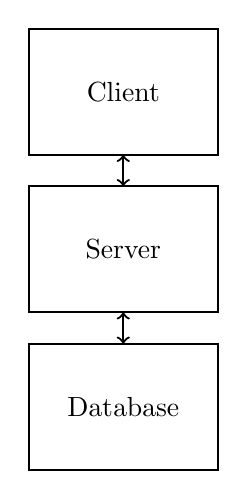
\begin{tikzpicture}[scale=0.8]
\draw[thick] (0,0) rectangle (3,2) node[pos=.5] {Client};
\draw[thick] (0,-2.5) rectangle (3,-0.5) node[pos=.5] {Server};
\draw[thick] (0,-5) rectangle (3,-3) node[pos=.5] {Database};
\draw[<->,thick] (1.5,0) -- (1.5,-0.5);
\draw[<->,thick] (1.5,-2.5) -- (1.5,-3);
\end{tikzpicture}
\end{columns}
\end{frame}

\begin{frame}{Client-Side Components}
\textbf{Frontend Technologies:}
\begin{itemize}
\item \textbf{HTML5} - Structure and Content
\item \textbf{CSS3} - Styling and Layout
\item \textbf{JavaScript} - Interactivity and Logic
\item \textbf{Frameworks:} React, Angular, Vue.js
\end{itemize}
\textbf{Security Considerations:}
\begin{itemize}
\item Cross-Site Scripting (XSS)
\item Content Security Policy (CSP)
\input validation
\item Secure cookie handling
\end{itemize}
\end{frame}

\begin{frame}{Server-Side Components}
\textbf{Backend Technologies:}
\begin{itemize}
\item \textbf{PHP} - Server-side scripting
\item \textbf{ASP.NET} - Microsoft web framework
\item \textbf{Node.js} - JavaScript runtime
\item \textbf{Python} - Django, Flask frameworks
\item \textbf{Java} - Spring Boot, JSP
\end{itemize}
\textbf{Security Aspects:}
\begin{itemize}
\item Authentication and Authorization
\item Session Management
\item Input Validation
\item Error Handling
\end{itemize}
\end{frame}

\begin{frame}{Database Layer}
\textbf{Database Types:}
\begin{itemize}
\item \textbf{SQL Databases:} MySQL, PostgreSQL, SQL Server
\item \textbf{NoSQL Databases:} MongoDB, Redis, Cassandra
\item \textbf{Object Storage:} Amazon S3, Google Cloud Storage
\end{itemize}
\textbf{Database Security:}
\begin{itemize}
\item SQL Injection Prevention
\item Access Control
\item Data Encryption
\item Backup and Recovery
\end{itemize}
\end{frame}

\begin{frame}{Component Interactions}
\begin{center}
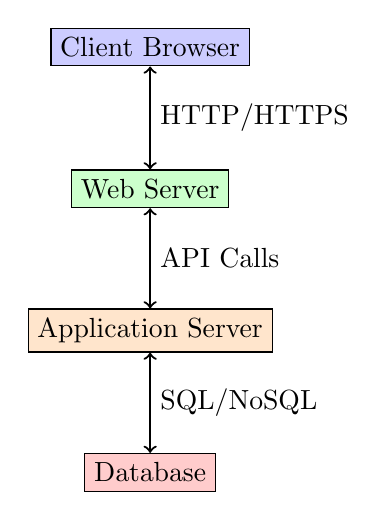
\begin{tikzpicture}[scale=0.9]
\node[draw, rectangle, fill=blue!20] (client) at (0,3) {Client Browser};
\node[draw, rectangle, fill=green!20] (web) at (0,1) {Web Server};
\node[draw, rectangle, fill=orange!20] (app) at (0,-1) {Application Server};
\node[draw, rectangle, fill=red!20] (db) at (0,-3) {Database};

\draw[<->, thick] (client) -- (web) node[midway, right] {HTTP/HTTPS};
\draw[<->, thick] (web) -- (app) node[midway, right] {API Calls};
\draw[<->, thick] (app) -- (db) node[midway, right] {SQL/NoSQL};
\end{tikzpicture}
\end{center}
\textbf{Communication Protocols:}
\begin{itemize}
\item HTTP/HTTPS for client-server
\item RESTful APIs for server-server
\item WebSockets for real-time communication
\end{itemize}
\end{frame}

\begin{frame}[fragile]{Common Web Technologies}
\textbf{Frontend Technologies:}
\begin{lstlisting}[language=HTML]
<!DOCTYPE html>
<html>
<head>
    <title>Secure Web App</title>
    <meta charset="UTF-8">
    <meta http-equiv="X-UA-Compatible" content="IE=edge">
</head>
<body>
    <script src="app.js"></script>
</body>
</html>
\end{lstlisting}
\end{frame}

\begin{frame}{Security Architecture Principles}
\textbf{Core Principles:}
\begin{enumerate}
\item \textbf{Defense in Depth}
\begin{itemize}
\item Multiple security layers
\item Redundant security controls
\end{itemize}
\item \textbf{Least Privilege}
\begin{itemize}
\item Minimal required permissions
\item Role-based access control
\end{itemize}
\item \textbf{Fail Secure}
\begin{itemize}
\item Default deny approach
\item Secure by default configuration
\end{itemize}
\end{enumerate}
\end{frame}

\begin{frame}{Hands-on Lab: Architecture Analysis}
\textbf{Lab Objectives:}
\begin{itemize}
\item Identify components in a web application
\item Map data flow between components
\item Identify potential security vulnerabilities
\item Recommend security improvements
\end{itemize}
\textbf{Lab Tasks:}
\begin{enumerate}
\item Analyze provided web application architecture
\item Document component interactions
\item Identify security gaps
\item Create security improvement plan
\end{enumerate}
\end{frame}

\section{Day 2: Web Application Threats and OWASP Top 10}

\begin{frame}{Day 2: Agenda}
\begin{enumerate}
\item \textbf{Morning Session (4 hours)}
\begin{itemize}
\item Common Web Application Threats
\item OWASP Top 10 Overview
\item Injection Attacks
\item Broken Authentication
\end{itemize}
\item \textbf{Afternoon Session (4 hours)}
\begin{itemize}
\item Sensitive Data Exposure
\item XML External Entities (XXE)
\item Broken Access Control
\item Security Misconfiguration
\item Hands-on Lab: Threat Analysis
\end{itemize}
\end{enumerate}
\end{frame}

\begin{frame}{Common Web Application Threats}
\textbf{Threat Categories:}
\begin{itemize}
\item \textbf{Injection Attacks}
\begin{itemize}
\item SQL Injection
\item Command Injection
\item LDAP Injection
\end{itemize}
\item \textbf{Cross-Site Scripting (XSS)}
\begin{itemize}
\item Stored XSS
\item Reflected XSS
\item DOM-based XSS
\end{itemize}
\item \textbf{Cross-Site Request Forgery (CSRF)}
\item \textbf{Security Misconfiguration}
\end{itemize}
\end{frame}

\begin{frame}{OWASP Top 10 Overview}
\begin{table}
\centering
\small
\begin{tabular}{ll}
\toprule
\textbf{Rank} & \textbf{Risk} \\
\midrule
A01:2021 & Broken Access Control \\
A02:2021 & Cryptographic Failures \\
A03:2021 & Injection \\
A04:2021 & Insecure Design \\
A05:2021 & Security Misconfiguration \\
A06:2021 & Vulnerable and Outdated Components \\
A07:2021 & Identification and Authentication Failures \\
A08:2021 & Software and Data Integrity Failures \\
A09:2021 & Security Logging and Monitoring Failures \\
A10:2021 & Server-Side Request Forgery (SSRF) \\
\bottomrule
\end{tabular}
\end{table}
\end{frame}

\begin{frame}[fragile]{Injection Attacks}
\textbf{SQL Injection Example:}
\begin{lstlisting}[language=SQL]
-- Vulnerable code
String query = "SELECT * FROM users WHERE username = '" + username + "' AND password = '" + password + "'";

-- Malicious input
username: admin' --
password: anything

-- Resulting query
SELECT * FROM users WHERE username = 'admin' --' AND password = 'anything'
\end{lstlisting}
\textbf{Prevention:}
\begin{itemize}
\item Use parameterized queries
\item Input validation
\item Least privilege database access
\end{itemize}
\end{frame}

\begin{frame}{Broken Authentication}
\textbf{Common Issues:}
\begin{itemize}
\item Weak password policies
\item Insecure session management
\item Missing multi-factor authentication
\item Credential stuffing attacks
\end{itemize}
\textbf{Mitigation Strategies:}
\begin{itemize}
\item Implement strong password requirements
\item Use secure session tokens
\item Enable MFA
\item Implement account lockout policies
\item Monitor for suspicious login attempts
\end{itemize}
\end{frame}

\begin{frame}{Sensitive Data Exposure}
\textbf{Types of Sensitive Data:}
\begin{itemize}
\item Personal identifiable information (PII)
\item Financial data
\item Authentication credentials
\item Intellectual property
\end{itemize}
\textbf{Protection Measures:}
\begin{itemize}
\item Data encryption at rest and in transit
\item Secure storage practices
\item Data masking and tokenization
\item Access controls
\item Regular security audits
\end{itemize}
\end{frame}

\begin{frame}[fragile]{XML External Entities (XXE)}
\textbf{Vulnerable XML Code:}
\begin{lstlisting}[language=XML]
<?xml version="1.0" encoding="ISO-8859-1"?>
<!DOCTYPE foo [
<!ELEMENT foo ANY >
<!ENTITY xxe SYSTEM "file:///etc/passwd" >]>
<foo>&xxe;</foo>
\end{lstlisting}
\textbf{Prevention:}
\begin{itemize}
\item Disable external entity processing
\item Use secure XML parsers
\item Validate XML input
\item Implement input sanitization
\end{itemize}
\end{frame}

\begin{frame}{Broken Access Control}
\textbf{Access Control Issues:}
\begin{itemize}
\item Insecure direct object references
\item Missing access control checks
\item Privilege escalation
\item Insecure object references
\end{itemize}
\textbf{Security Best Practices:}
\begin{itemize}
\item Implement role-based access control (RBAC)
\item Validate all user inputs
\item Use access control lists (ACLs)
\item Implement proper authorization checks
\item Regular access reviews
\end{itemize}
\end{frame}

\begin{frame}{Security Misconfiguration}
\textbf{Common Misconfigurations:}
\begin{itemize}
\item Default credentials
\item Verbose error messages
\item Unnecessary services enabled
\item Missing security headers
\item Insecure server configurations
\end{itemize}
\textbf{Prevention:}
\begin{itemize}
\item Regular security audits
\item Automated security scanning
\item Secure configuration baselines
\item Change default credentials
\item Implement security logging
\end{itemize}
\end{frame}

\begin{frame}{Hands-on Lab: Threat Analysis}
\textbf{Lab Objectives:}
\begin{itemize}
\item Identify vulnerabilities in web applications
\item Assess risk levels of identified threats
\item Develop mitigation strategies
\item Create security testing reports
\end{itemize}
\textbf{Lab Tasks:}
\begin{enumerate}
\item Analyze vulnerable web applications
\item Document identified vulnerabilities
\item Prioritize risks based on impact
\item Create remediation plans
\end{enumerate}
\end{frame}

\section{Day 3: Web Application Hacking Methodology and Tools}

\begin{frame}{Day 3: Agenda}
\begin{enumerate}
\item \textbf{Morning Session (4 hours)}
\begin{itemize}
\item Web Application Hacking Methodology
\item Reconnaissance Techniques
\item Scanning and Enumeration
\item Exploitation Methods
\end{itemize}
\item \textbf{Afternoon Session (4 hours)}
\begin{itemize}
\item Post-Exploitation Techniques
\item Webhooks and Web Shells
\item Web API Security
\item Hands-on Lab: Practical Hacking
\end{itemize}
\end{enumerate}
\end{frame}

\begin{frame}{Web Application Hacking Methodology}
\textbf{Hacking Lifecycle:}
\begin{enumerate}
\item \textbf{Reconnaissance}
\begin{itemize}
\item Information gathering
\item Target identification
\item Attack surface mapping
\end{itemize}
\item \textbf{Scanning}
\begin{itemize}
\item Vulnerability scanning
\item Port scanning
\item Service enumeration
\end{itemize}
\item \textbf{Enumeration}
\begin{itemize}
\item Directory traversal
\item Information disclosure
\item Fingerprinting
\end{itemize}
\item \textbf{Exploitation}
\begin{itemize}
\item Vulnerability exploitation
\item Privilege escalation
\item Persistence
\end{itemize}
\end{enumerate}
\end{frame}

\begin{frame}{Reconnaissance Techniques}
\textbf{Passive Reconnaissance:}
\begin{itemize}
\item Google Dorking
\item Social media analysis
\item Public records search
\item DNS enumeration
\item WHOIS lookup
\end{itemize}
\textbf{Active Reconnaissance:}
\begin{itemize}
\item Port scanning
\item Service enumeration
\item Banner grabbing
\item Directory brute-forcing
\item Subdomain enumeration
\end{itemize}
\end{frame}

\begin{frame}[fragile]{Scanning and Enumeration}
\textbf{Nmap Scanning Examples:}
\begin{lstlisting}[language=bash]
# Basic port scan
nmap -sS target.com

# Service version detection
nmap -sV target.com

# Aggressive scan
nmap -A target.com

# UDP scanning
nmap -sU target.com
\end{lstlisting}
\textbf{Enumeration Tools:}
\begin{itemize}
\item Dirb/Dirbuster for directory enumeration
\item Nikto for web server scanning
\item OWASP ZAP for web application scanning
\item Burp Suite for proxy and scanning
\end{itemize}
\end{frame}

\begin{frame}{Exploitation Methods}
\textbf{Common Exploitation Techniques:}
\begin{itemize}
\item \textbf{SQL Injection}
\begin{itemize}
\item Union-based injection
\item Error-based injection
\item Blind injection
\end{itemize}
\item \textbf{Cross-Site Scripting (XSS)}
\begin{itemize}
\item Stored XSS attacks
\item Reflected XSS attacks
\item DOM-based XSS
\end{itemize}
\item \textbf{File Upload Vulnerabilities}
\begin{itemize}
\item File type validation bypass
\item Directory traversal
\item Remote code execution
\end{itemize}
\end{itemize}
\end{frame}

\begin{frame}{Post-Exploitation Techniques}
\textbf{Post-Exploitation Activities:}
\begin{itemize}
\item \textbf{Persistence}
\begin{itemize}
\item Backdoor creation
\item User account creation
\item Scheduled tasks
\end{itemize}
\item \textbf{Privilege Escalation}
\begin{itemize}
\item Exploiting misconfigurations
\item Weak permissions
\item Vulnerable services
\end{itemize}
\item \textbf{Data Exfiltration}
\begin{itemize}
\item Data extraction
\item Information gathering
\item Covering tracks
\end{itemize}
\end{itemize}
\end{frame}

\begin{frame}{Webhooks and Web Shells}
\textbf{Webhooks:}
\begin{itemize}
\item HTTP callbacks for real-time communication
\item Used for integration between services
\item Security considerations:
\begin{itemize}
\item Authentication and authorization
\item Input validation
\item Rate limiting
\end{itemize}
\end{itemize}
\textbf{Web Shells:}
\begin{itemize}
\item Malicious scripts for remote access
\item Common types:
\begin{itemize}
\item PHP web shells
\item ASP web shells
\item JSP web shells
\end{itemize}
\item Detection and prevention:
\begin{itemize}
\item File integrity monitoring
\item Web application firewalls
\item Regular security audits
\end{itemize}
\end{itemize}
\end{frame}

\begin{frame}{Web API Security}
\textbf{Web API Security Challenges:}
\begin{itemize}
\item Authentication and authorization
\item Rate limiting and throttling
\item Input validation
\item Data protection
\item API versioning
\end{itemize}
\textbf{Security Best Practices:}
\begin{itemize}
\item Implement OAuth 2.0/OpenID Connect
\item Use API gateways
\item Implement rate limiting
\item Monitor API usage
\item Regular security testing
\end{itemize}
\end{frame}

\begin{frame}[fragile]{Hands-on Lab: Practical Hacking}
\textbf{Lab Objectives:}
\begin{itemize}
\item Apply hacking methodology in practice
\item Use security tools effectively
\item Identify and exploit vulnerabilities
\item Document findings and recommendations
\end{itemize}
\textbf{Lab Environment:}
\begin{lstlisting}[language=bash]
# Setup vulnerable applications
docker run -p 8080:80 vulnerable-web-app
docker run -p 8081:80 dvwa

# Security tools to use
- Burp Suite
- OWASP ZAP
- Metasploit
- Nmap
- SQLMap
\end{lstlisting}
\end{frame}

\section{Day 4: Security Testing, Mitigation, and Best Practices}

\begin{frame}{Day 4: Agenda}
\begin{enumerate}
\item \textbf{Morning Session (4 hours)}
\begin{itemize}
\item Security Testing Methodologies
\item Vulnerability Assessment
\item Penetration Testing
\item Security Code Review
\end{itemize}
\item \textbf{Afternoon Session (4 hours)}
\begin{itemize}
\item Security Best Practices
\item Incident Response Planning
\item Security Monitoring
\item Hands-on Lab: Security Implementation
\end{itemize}
\end{enumerate}
\end{frame}

\begin{frame}{Security Testing Methodologies}
\textbf{Types of Security Testing:}
\begin{itemize}
\item \textbf{Vulnerability Assessment}
\begin{itemize}
\item Automated scanning
\item Vulnerability identification
\item Risk prioritization
\end{itemize}
\item \textbf{Penetration Testing}
\begin{itemize}
\item Manual testing
\item Exploitation attempts
\item Real-world attack simulation
\end{itemize}
\item \textbf{Security Code Review}
\begin{itemize}
\item Static analysis
\item Dynamic analysis
\item Manual code inspection
\end{itemize}
\end{itemize}
\end{frame}

\begin{frame}{Vulnerability Assessment}
\textbf{Assessment Process:}
\begin{enumerate}
\item \textbf{Planning and Scoping}
\begin{itemize}
\item Define scope and objectives
\item Identify assets and systems
\item Set assessment criteria
\end{itemize}
\item \textbf{Information Gathering}
\begin{itemize}
\item Asset discovery
\item Network mapping
\item Service enumeration
\end{itemize}
\item \textbf{Vulnerability Scanning}
\begin{itemize}
\item Automated scanning tools
\item Manual verification
\item False positive identification
\end{itemize}
\item \textbf{Reporting and Remediation}
\begin{itemize}
\item Risk assessment
\item Prioritization
\item Remediation planning
\end{itemize}
\end{enumerate}
\end{frame}

\begin{frame}{Penetration Testing}
\textbf{Penetration Testing Methodology:}
\begin{enumerate}
\item \textbf{Pre-engagement}
\begin{itemize}
\item Scope definition
\item Rules of engagement
\item Resource planning
\end{itemize}
\item \textbf{Reconnaissance}
\begin{itemize}
\item Passive information gathering
\item Active scanning
\item Target analysis
\end{itemize}
\item \textbf{Exploitation}
\begin{itemize}
\item Vulnerability identification
\item Exploitation attempts
\item Post-exploitation activities
\end{itemize}
\item \textbf{Reporting}
\begin{itemize}
\item Findings documentation
\item Risk assessment
\item Remediation recommendations
\end{itemize}
\end{enumerate}
\end{frame}

\begin{frame}{Security Code Review}
\textbf{Code Review Areas:}
\begin{itemize}
\item \textbf{Input Validation}
\begin{itemize}
\item SQL injection prevention
\item XSS protection
\item File upload security
\end{itemize}
\item \textbf{Authentication and Authorization}
\begin{itemize}
\item Session management
\item Access control
\item Password handling
\end{itemize}
\item \textbf{Error Handling}
\begin{itemize}
\item Information disclosure
\item Stack traces
\item Error messages
\end{itemize}
\item \textbf{Data Protection}
\begin{itemize}
\item Encryption
\item Secure storage
\item Data transmission
\end{itemize}
\end{itemize}
\end{frame}

\begin{frame}{Security Best Practices}
\textbf{Development Security:}
\begin{itemize}
\item Implement secure coding standards
\item Use security-focused frameworks
\item Regular code reviews
\item Security testing in CI/CD pipeline
\end{itemize}
\textbf{Infrastructure Security:}
\begin{itemize}
\item Principle of least privilege
\item Regular security updates
\item Network segmentation
\item Monitoring and logging
\end{itemize}
\textbf{Operational Security:}
\begin{itemize}
\item Security awareness training
\item Incident response planning
\item Regular security audits
\item Compliance with standards
\end{itemize}
\end{frame}

\begin{frame}{Incident Response Planning}
\textbf{Incident Response Lifecycle:}
\begin{enumerate}
\item \textbf{Preparation}
\begin{itemize}
\item Develop incident response plan
\item Establish response team
\item Create playbooks
\end{itemize}
\item \textbf{Detection and Analysis}
\begin{itemize}
\item Monitoring and alerting
\item Incident classification
\item Impact assessment
\end{itemize}
\item \textbf{Containment, Eradication, and Recovery}
\begin{itemize}
\item Containment strategies
\item Root cause analysis
\item System restoration
\end{itemize}
\item \textbf{Post-Incident Activity}
\begin{itemize}
\item Lessons learned
\item Plan updates
\item Training improvements
\end{itemize}
\end{enumerate}
\end{frame}

\begin{frame}{Security Monitoring}
\textbf{Monitoring Components:}
\begin{itemize}
\item \textbf{Log Management}
\begin{itemize}
\item Centralized logging
\item Log correlation
\item Retention policies
\end{itemize}
\item \textbf{Security Information and Event Management (SIEM)}
\begin{itemize}
\item Real-time monitoring
\item Alerting and notifications
\item Compliance reporting
\end{itemize}
\item \textbf{Intrusion Detection/Prevention Systems (IDS/IPS)}
\begin{itemize}
\item Network-based monitoring
\item Host-based monitoring
\item Behavioral analysis
\end{itemize}
\end{itemize}
\end{frame}

\begin{frame}{Hands-on Lab: Security Implementation}
\textbf{Lab Objectives:}
\begin{itemize}
\item Implement security controls
\item Configure security tools
\item Test security measures
\item Create security documentation
\end{itemize}
\textbf{Lab Tasks:}
\begin{enumerate}
\item Configure web application firewall
\item Implement input validation
\item Set up monitoring and alerting
\item Create security policies and procedures
\item Test incident response procedures
\end{enumerate}
\end{frame}

\begin{frame}{Training Summary}
\textbf{Key Takeaways:}
\begin{itemize}
\item Web application security is crucial for protecting data and systems
\item Understanding architecture helps identify security vulnerabilities
\item OWASP Top 10 provides a framework for addressing common threats
\item Proper methodology and tools are essential for effective security testing
\item Security should be integrated throughout the development lifecycle
\end{itemize}
\textbf{Next Steps:}
\begin{itemize}
\item Apply learned concepts in real-world scenarios
\item Stay updated with emerging threats and technologies
\item Implement security best practices in your organization
\item Continuous learning and improvement
\end{itemize}
\end{frame}

\begin{frame}{Thank You}
\begin{center}
\Large{Questions?}\\
\vspace{1cm}
\normalsize{Contact: security-team@organization.com}\\
\vspace{0.5cm}
\small{Additional Resources:}\\
\small{OWASP Foundation: https://owasp.org}\\
\small{OWASP Top 10: https://owasp.org/www-project-top-ten/}
\end{center}
\end{frame}

\end{document}